\documentclass[12pt]{article}

\usepackage[paperheight=1.75in,paperwidth=4in,top=.25in,bottom=0in,right=0in,left=0in]{geometry}
%fancy math symbols
\usepackage{amsmath}
\usepackage{amssymb}
\usepackage{cancel}
%fancy font
%\usepackage{pxfonts}
\usepackage[T1]{fontenc}
%DAGs
\usepackage{tikz}
\usetikzlibrary{arrows,positioning,snakes,calc,shapes}
\tikzset{>=latex}
\usepackage{subfig}
\captionsetup[subfloat]{position = top, font = large} % For sub-figure captions
\renewcommand{\thesubfigure}{\normalsize\Alph{subfigure})}
\usepackage{float}

\begin{document}
  \begin{figure}[H]
    \begin{center}
     
    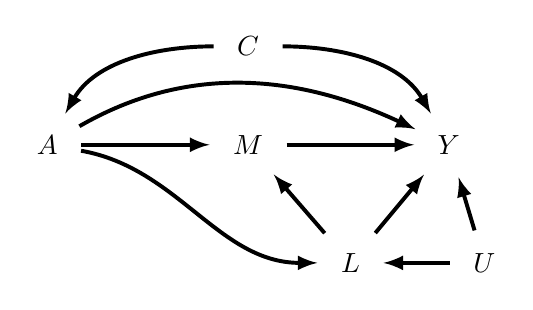
\begin{tikzpicture}
    
    \node [align=center] (m) at (0,0) {$M$};
    \node [align=center] (x) at (-2.55,0) {$A$};
    \node [align=center] (y) at (2.55,0) {$Y$};
    \node [align=center] (c1) at (0,1.25) {$C$};
    \node [align=center] (c3) at (1.3,-1.5) {$L$};
    \node [align=center] (u) at (3,-1.5) {$U$};
    
    \begin{scope}[line width=.05cm,shorten >= 5pt, shorten <= 5pt]
    \draw[->,color=black] (x) to (m);
    \draw[->,color=black] (m) to (y);
    \draw[->,color=black] (x) to [out=350,in=180] (c3);
    \draw[->,color=black] (x) to [out=30,in=155] (y);
    \draw[->,color=black] (c1) to [out=0,in=120] (y);
    \draw[->,color=black] (c1) to [out=180,in=60] (x);
    %\draw[->,color=black] (c2) to (x);
    %\draw[->,color=black] (c2) to (m);
    \draw[->,color=black] (c3) to (m);
    \draw[->,color=black] (c3) to (y);
    \draw[->,color=black] (u) to (y);
    \draw[->,color=black] (u) to (c3);
    \end{scope}
    
    \end{tikzpicture}
    \end{center}
  \end{figure}
\end{document}